\documentclass[]{scrreprt}

%Dokument auf Deutsch umstellen und Zeichensätze nachladen
\usepackage[utf8]{inputenc}
\usepackage[ngerman]{babel}
\usepackage[T1]{fontenc}

%Absätze einrücken
\usepackage[parfill]{parskip}

\usepackage{graphicx}

\usepackage[citecolor = black,colorlinks=true,linkcolor=black,urlcolor=black]{hyperref}

% enthält die konfiguration für das listings package
\usepackage{listings}
\usepackage{xcolor}
\lstset{language=Java}
\definecolor{lst_light_grey}
{rgb}{0.95,0.95,0.95}
\definecolor{lst_dark_grey}
{rgb}{0.8,0.8,0.8}
\definecolor{lst_highlight}
{rgb}{0,0,0.6}
\definecolor{lstgreen}
{rgb}{0,0.6,0}
\definecolor{lstmauve}
{rgb}{0.58,0,0.82}
\lstset{ %
basicstyle=\small\ttfamily, %
backgroundcolor=\color{lst_light_grey}, %
captionpos=b, %
commentstyle=\color{lstgreen}, %
frame=single, %
tabsize=2, %
%
keywordstyle=\color{lst_highlight}, %
%
numbers=left, %
%
numberstyle=\scriptsize \color{lst_dark_grey}, %
%
rulecolor=\color{lst_dark_grey}, %
}
% additional highlighted keywords
\lstset { emph= {%
var, function %
}, emphstyle={\color{lst_highlight}}%
}
\lstset{showstringspaces=false}

%Metadaten für Titelblatt
\author{Klaus}
\title{Lebendiges Minimalbeispiel}
\date{6. Juli 2097}
\begin{document}

\maketitle %erzeugt Titelseite

\tableofcontents %erzeugt Inhaltsverzeichnis

\listoffigures %Abbildungsverzeichnis

\chapter{Einführendes Beispiel}

\section{Blubbb}

Text mit Ö und Ü.

\chapter{Zwischenschicht}

Kein sinnvoller Text.

\pagenumbering{Roman}

\chapter{42}
\label{ch:42}



\section{Hallo Welt!}
\tiny
Ich bin der \textbf{tolle} \textsc{Text} auf der ersten Seite! 
\normalsize

Testtexte sind toll! Und Absätze sind noch viel besser, so sie denn mit viel Text gefüllt sind. Daher produziere ich gerade viel Text als Platzhalter, der keinen Sinn ergibt.

Ich verweise auf das Kapitel \ref{ch:42}.

\subsection{Unterüberschrift}

Das ist ein langer Beispieltext.

\subsubsection{Unter der Unterüberschrift}

\begin{figure}[h]
\centering
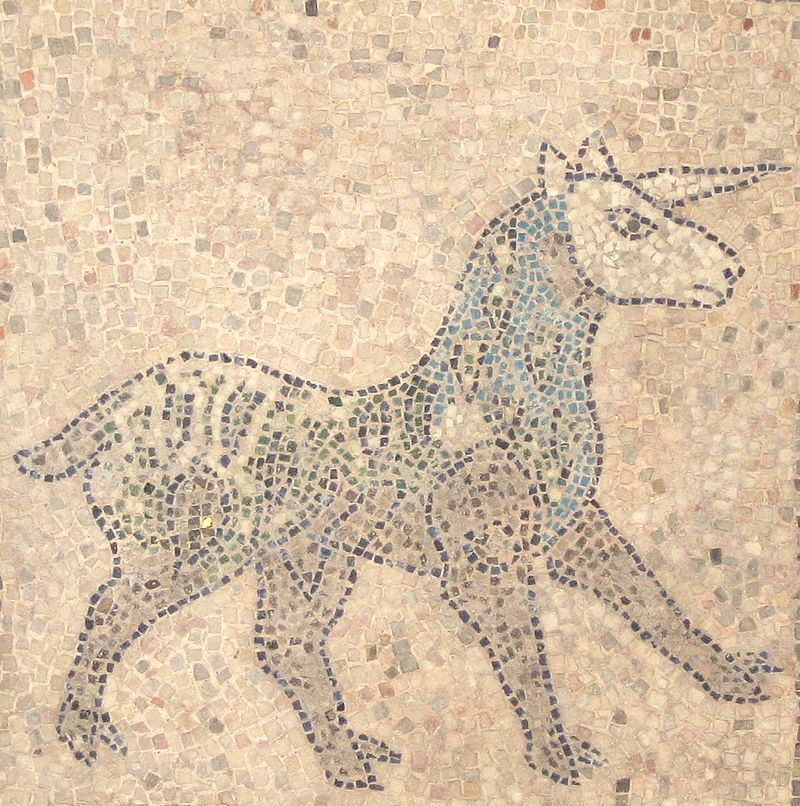
\includegraphics[scale=0.2]{einhorn.jpg}
\caption{Ein Einhorn}
\label{fig:einhorn}
\end{figure}

\section{Minipage Beispiel}

Noch etwas Text.

\begin{figure}[h!]
\begin{minipage}[hbt]{0.5\textwidth}
\centering
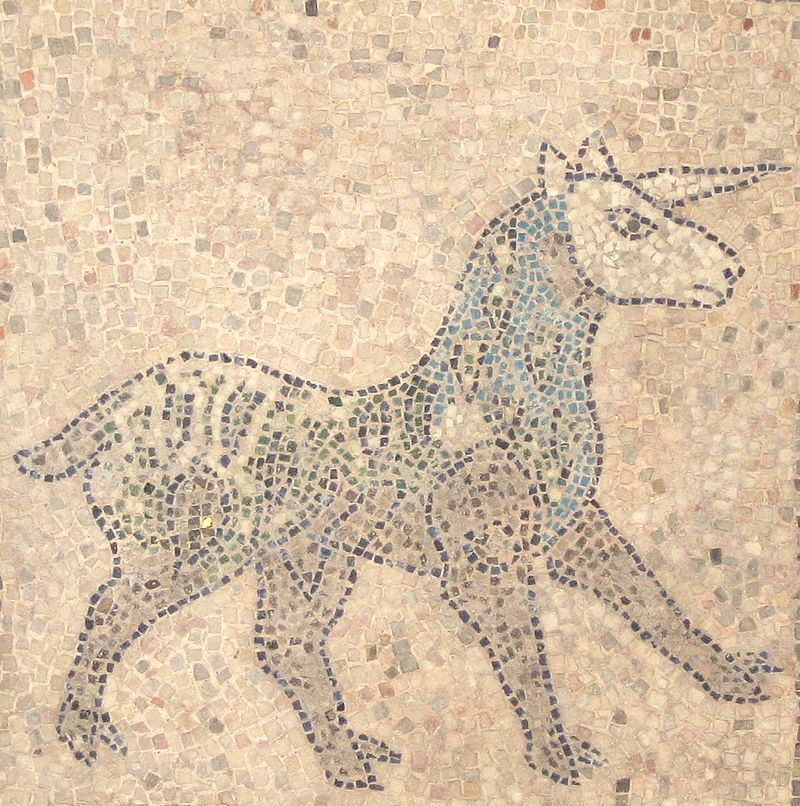
\includegraphics[width=0.9\textwidth]{einhorn.jpg}
\caption{Ein Einhorn}
\label{fig:einhorn1}
\end{minipage}
\hfil
\begin{minipage}[hbt]{0.5\textwidth}
\centering
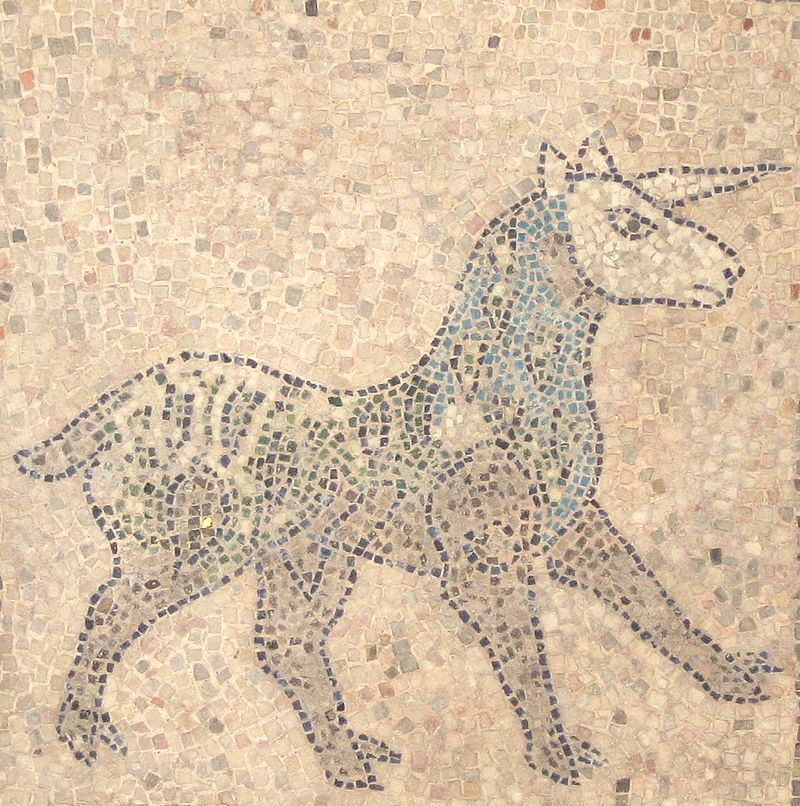
\includegraphics[width=0.9\textwidth]{einhorn.jpg}
\caption{Noch ein Einhorn}
\label{fig:einhorn2}
\end{minipage}
\end{figure}

\section{Listenbeispiel}

\begin{itemize}
\item Stichpunkt 1
\item Einschub
\begin{itemize}
\item Hallo
\item Welt
\end{itemize}

\item Stichpunkt 2
\item Neuer toller Stichpunkt
\end{itemize}

\begin{description}
\item [Definition] Ich definiere mich selbst.
\item [Andere Definition] Ich definiere mich auch selbstständig. Und ich gehe über mehrere Zeilen, weil ich eine lange Definition bin.
\end{description}

\section{Tabellen}

\begin{table}[h]
\centering
\begin{tabular}{|c||l|r|}
\hline
Stadt & Land & Fluss \\
\hline
Buxtehude & Österreich & Mississippi\\
\hline
Görlitz & Nepal & Neiße\\
\hline
\end{tabular}
\caption{Ein beliebtes Spiel}
\label{tab:stadt}
\end{table}

In diesem Text referenziere ich eine Tabelle. Diese ist Tabelle \ref{tab:stadt}.

Eine Formel wäre cool! $a^2 + b^2 = c^2$
\[ Obstsalat_4 = \frac{Apfel}{Birnen} \]

\section{Listings}

\begin{lstlisting}[caption=Example, label=meinCode]
public class Example {
public static void main(String...args){
System.out.println("hello World");
}
}
\end{lstlisting}


In diesem Text referenziere ich auf Listing \ref{meinCode} und zeige ein Beispiel\footnote{Anmerkung des Autors}. Und ein Beispiel für Worttrennung: Multi-Groß-Konzern-Warenketten-Vertriebs-Abteilungs-Leiterbereit\-schafts-Büro

\end{document}